\documentclass{article}
\usepackage{graphicx} % Required for inserting images
\usepackage{hyperref} %hyperlinked all references and pages
\usepackage[backend=biber, style=apa]{biblatex}
\usepackage[utf8]{inputenc}
\usepackage{caption}
\usepackage{amsmath}
\usepackage{booktabs}
\addbibresource{thesis.bib}
% This does the same for the figures.
\setcounter{tocdepth}{2}


\begin{document}
% THESIS COVER PAGE

% Choose Honors/Senior and Arts/Science below as appropriate.

\vspace*{4cm} 
% LaTeX will remove blank space at the start or end of a page,
%   but the asterisk prevents this.

\centerline{\LARGE \textbf{Unemployment insurance take-up on social networks}}
\bigskip\bigskip
\centerline{\Large  A Senior Thesis}
%\centerline{\Large  A Senior Thesis}
\medskip
\centerline{\Large Presented to the Department of Economics}
\medskip
\centerline{\Large Bates College}
\medskip
\centerline{\Large in partial fulfillment of the requirements for the}
\medskip
\centerline{\Large Degree of Bachelor of Arts}
%\centerline{\Large Degree of Bachelor of Science}
\medskip
\centerline{\Large by}
\medskip
\centerline{\Large Yuhao Zhao}
\medskip
\centerline{\Large Lewiston, Maine}
\medskip
\centerline{\Large April 1, 2024}


\centerline{}
\newpage



\tableofcontents

\newcounter{pnumb}                     	% Save page number of intro material
\setcounter{pnumb}{\value{page}}       	% so that numbering will be consecutive.
                          	% Begin body
\setcounter{page}{\value{pnumb}}       	% with consecutive page numbering
\newpage
\section{Introduction}

%During periods of economic turmoil, people often rely on their friends and family, or their social network to provide them with informal financial and in-kind support. They may receive this informal support alongside formal social insurance programs like unemployment insurance (UI) compensation. Alternatively, informal support may act as a substitute for social insurance programs, which are often cumbersome to navigate and replace a fraction of lost earnings (cite). Such substitution could explain why TK percent of eligible unemployed workers in the United States did not enroll in unemployment insurance (UI) benefits in YEAR (cite).


When thinking about the resources people possess, it's often inevitable to talk about individual's social relationships.  Why should do we care about social relationships? At its core, it is about the subtle but important resources embedded in social relationships or networks. Like other forms of capitals, social capitals often plays essential roles in shaping how people make uses of other forms of capitals/resources through linkages and structures of social networks. Social networks permeate our social and economic lives. Not only just because of the salience of networks have draw people's eyes in recent decades, the facts that economists, or more broadly speaking the social scientists, cannot igore the social interactions across in trying to understand the human social behaviors. They play a central role in the transmission of information about job opportunities, and are critical to the trade of many goods and services. Social networks are also important in determining how diseases spread, which products we buy, which languages we speak, how we vote, as well as whether or not we decide to become criminals, how much education we obtain, and our likelihood of succeeding professionally.

Social capital can also reduce information frictions and search costs for workers and firms, helping the labor market function more efficiently. Furthermore, social capitals can also be treated as a source of informal insurance or risk-sharing mechanism when it comes to massive layoffs and transition period from unemployment to re-employment. During periods of economic turmoil, people often rely on their friends and family, or their social network to provide them with informal financial and in-kind support. They may receive this informal support alongside formal social insurance programs like unemployment insurance (UI) compensation. In developing countries where formal insurance institutions are inaccessible and incomplete, social networks provide robust informal insurance in small tight-knit communities \cite{microfinance}. Alternatively, informal support may act as a substitute for social insurance programs, which are often cumbersome to navigate and replace a fraction of lost earnings (cite). Such substitution could explain why 30 percent of UI total expenditure are "unclaimed" UI benefits belongs to eligible unemployed workers \cite{gap_takeup}.

And my research focus comes in when I are getting interested in gap between the claimed unemployment insurance and the total unemployment group. From the workers' side, the significant amount of "unclaimed" benefits indicate possible costs from various sources that can not be overlooked--like fixed up-front administrative costs, stigma cost and cost related to eligibility verification. However, shortage of income benefits of unemployed people-both insured and uninsured should be filled up through different channels when people are on the period of seeking re-employment. 


%In many studies of local social networks across developing countries, researchers have found significant results of informal insurance system that embedded in people's social networks where insurance institutions are not been developed or much less accessible. Micro-level public finance system are established and evolved from simple cash transfer to risk-sharing premium are diffused across less-developed rural areas\@.
Nonetheless, I am more curious about more institutional-developed setting where people have access to public insurances through institutions but still manage or obtain resources through social capital accumulations when costs of the public resources are high. Here I envision the importance of social capitals in filling the gap for uninsured unemployed population across regions in United States particularly in NY area. In examining the relationship between social capital aggregation and take-up of formal unemployment insurance benefits, this paper is organized as follows. Next section gives an overview of relevant literature and how do them bridge into this work. Rest of sections focus on data collection, method, result and finally discussion upon this work.


I think this area of research matters for people interested in labor economics, especially at the intersections of unemployment insurance and social network effect on regional economic performance. It will draw interests from people who also interested in public policy and local community engagement in understanding and intervening in institutional insurance policies based on regional social capital differences. And my thesis adds values in mainly two major ways: 
\begin{itemize}
\item The first is bridging unemployment insurance data with recent empirical project on social capitals that measured from national-wide users on large online social networks.

\item The second is exploring the social network effects on UI insurance program--seldom work particularly focus on this specific track; I will go over some relevant literature in study how social capitals related to unemployment risks and other metric performance.
 
\end{itemize}



\section{Background}
%KGC: Also, group literature by method or finding/subtopic. Tell me a story of the literature. What can I learn from each sub-part of the literature?_
%structure of storyline: social captial and network definition; network effects on unemployment; informal support and unemployment insurance; social networks/capital as channel of informal support; 

Social capital is defined as the networks of relationship among people who live and work in a particular society. In another term, social capital is the aggregated and abstract term for values embedded in one's social networks. Although social capitals are abstract concepts that often appear qualitatively, we can still measure and even differentiating forms of social capitals by network-based measures \cite{Jackson2020}.
%Quantitatively, when we are trying to measure the social capitals, not like physical capital or human capital, we often face problems with quantifying the intangible feature of it: values/weights of links to friends from different social-economic backgrounds, degree of clustering of different sub-communities within the general network, and so on.  
In \cite{jackson2014networks}, he extensively discussed how networks play roles in understanding economic behaviors in variety of ways. Particularly, he talks about how measures of network property at different scales (like network density, centrality, local clustering) impact behaviors throughout the networks. \cite{informalshare_local} found that centrality is positively correlated with consumption volatility which indicating the informal insurance sharing from central agents to peripheral agents on networks. In \cite{hallsten2017social}, researchers have found the significant roles that social networks play in affecting the youth's unemployment risks through both occupational contact networks and friendship networks. Another paper \cite{freitag2011social} analyzed at macro-level relationship between regional social capital levels and number of unemployed people in European regions which shows that regional level aggregation of social capitals is negatively related to total number of unemployment. The previous work have set the tone for considering unemployment problems and measures of social capitals.

Studies have shown that people often use private transfers or other informal sources for risk-sharing and consumption-smoothing as substitute for formal insurance \cite{ligon2002informal}
\cite{rosenzweig1988risk} and interactions between informal insurances and formal insurance is pertinent to this work. In \cite{modelofcrowdingout}, researchers studied on crowding-out mechanism where crowding-out effect of formal insurance is not more than one-for-one for informal insurance, and hence the total risk coverage is not significantly reduced by formal insurance.
Another one works on a empirical project on sub-castes in rural India. They found that informal networks lower the demand for formal insurance only if the network indemnifies against aggregate risk, but not if its primary role is to insure
against farmer-specific losses (\cite{mobarak2012selling}). Therefore, it is fully reasonable for both insurance market and "moral economy" co-exist in all regions especially for under-developed areas.

Due to its connecting nature, social networks naturally serve as the basis of the provision of informal insurance or risk-sharing mechanism. Particularly, in developing countries and regions, formal insurance normally cannot provide good risk coverage which require people to rely more on various kind of informal risk-sharing mechanisms through friends and families including gift giving, shared meals, reciprocal interest-free credit and some land/work sharing \cite{coate1993reciprocity}. Researchers also provide theoretical support in understanding of informal support through social networks by connecting with graph theories: researchers found that stable networks as suitably “sparse” networks. Thickly and thinly connected networks tend to be stable, whereas intermediate degrees of connectedness jeopardize stability. People also explore the formation of risk-sharing network (a pattern of existing relations where agents can commit to sharing income) and validate that identical individuals can end up in different positions in a network and have different outcomes. These results may help to explain empirical findings that risk-sharing is often asymmetric. \cite{bloch2008informal}\cite{risksharing} 

In rural India, implemented micro-finance systems spread throughout social contact networks, increasing take-up of a formal institution  \cite{microfinance}. Another study shows the effects of UI benefit in the presence of informal sector: an increase in UI benefits received by short-run unemployed workers unambiguously increases the efforts of long-run unemployed workers to find a formal job\cite{informalsector}. Nonetheless, the measurement and studies of informal insurance in high-income countries have eluded researchers for a long period of time. But recently researchers have adopted data from P2P platform to start analyzing the informal insurance in developed areas. \cite{balyuk2021friends} studied the importance of real-time instant money transfers from friends and family to financially fragile consumers. In \cite{coombs2022crowding}, findings suggest that provision of formal insurance in US is not holding back the private insurance within people's social networks and within-network informal insurance varies locally. 

Since local level of resources including social capitals vary a lot and keeping the formal social insurance is important to health of labor market, I am interested in how does some aggregated social capital measures of social contact networks affect the take-up of formal unemployment insurance which might shed light on policy making in adjusting UI expenditure distribution across.






\section{Data and Method}

\subsection{Data}

\subsubsection{Data Description}

Our raw datasets consist of three major components: Social capital data, Unemployment data and Unemployment Insurance data.


The social capital statistics come from the large-scale data project \href{https://socialcapital.org}{The Social Capital Atlas} where the data are publicly available and ready for everyone to download at:\url{https://data.humdata.org/dataset/social-capital-atlas}. The dataset I am using is in the cross-section data form where first columns is each US county and other columns are specific statistics calculated or collected using privacy-protected Facebook data except population variables. The primary sample they use to construct these statistics consists of Facebook users aged between 25 and 44 who reside in the United States, were active on the Facebook platform at least once in the prior 30 days, have at least 100 U.S.-based Facebook friends, and have a non-missing residential ZIP code as of May 28, 2022. In this study, I am focusing on the NY state so that I have subsetted the social capital datasets within the NY area. And since we don't have the time-series data on how social contact network change, those measures that we included in analysis are all fixed across 2021-2022.

The Unemployment data I have collected is from \href{https://dol.ny.gov/local-area-unemployment-statistics}{New York Department of Labor's Local Area Unemployment Statistics (LAUS)} program where it provides publicly available datasets on monthly and annual employment, unemployment, labor force, and unemployment rate data for New York State, labor market regions, metropolitan areas, counties, workforce investment regions, and municipalities of at least 25,000 people. LAUS is a joint effort between New York State and the United States Bureau of Labor Statistics (BLS) and there is also dashboard for users/customers to play around and explore the data. Here I focus on the data spanning from 2021 to 2022. The raw unemployment data I downloaded is in panel data form which includes Year, Month, area name, employed, unemployed, labor force and unemployment rate variables and total 1488 observations in total. 

The UI data I have collected is from New York Department of Labor's \href{https://dol.ny.gov/local-area-unemployment-statistics}{Unemployment Insurance Data} where you will be able to look at information for benefits paid, beneficiaries and initial claims by region, industry, and program. Here I only collect the data span across 2021-2022 given that our social capital stats are calculated based on Facebook users' residential ZIP code as of May, 2022. The raw data I downloaded is in a time series but wide data form across 63 counties for every month in 2021-22. The original variables include number of beneficiaries and total amount of benefits. Below we first provide the variable descriptions of interested variables in this study (See Table \ref{variable descr}).



\begin{table}[h]
\centering
\begin{tabular}{|p{3.2cm}|p{8cm}|p{4cm}|}
\hline
\textbf{Variable Name} & \textbf{Description} & \textbf{ Unit of Measurement} \\ \hline
takeup & Monthly take-up (recipiency) rate by county & Proportion  \\ \hline
Avg\_takeup & Average of Monthly take-up (recipiency) rate by county in given year & Average proportion \\ \hline
ec\_county & The mean level of individual EC (economic connectedness) of low-SES (Socioeconomic status; for example, below-median) members of that community. &  \\ \hline
clustering\_county & The average fraction of an individual's friend pairs who are also friends with each other. & Average fraction of closed triangle out of individual's network \\ \hline
Volunteer\_rate\_county & The percentage of online social network users who are members of a group which is predicted to be about 'volunteering' or 'activism' based on group title and other group characteristics. & proportion \\ \hline
\end{tabular}
\caption{Description and Measurement for Variables}
\label{variable descr}
\end{table}


\begin{figure}[h]
\begin{minipage}{0.5\textwidth}
    \centering
    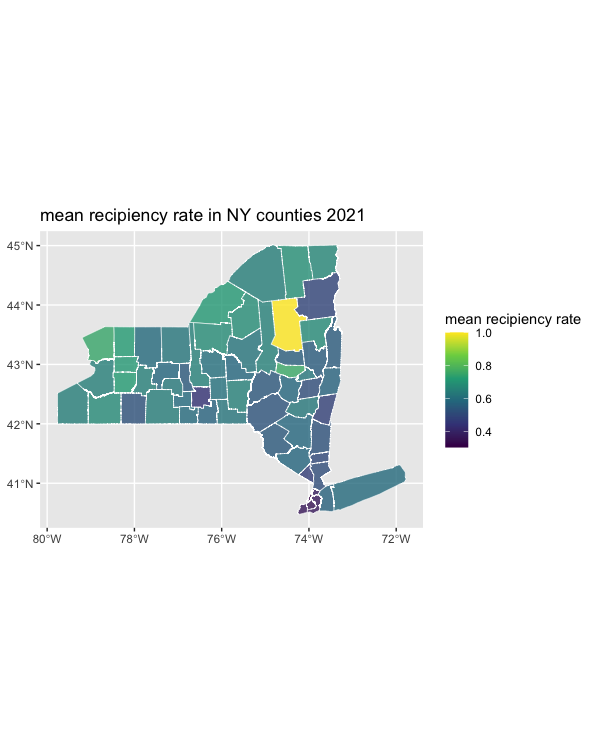
\includegraphics[width=\textwidth]{mean_recip_NY_2021.png} % First figure
  \end{minipage}\hfill
  \begin{minipage}{0.5\textwidth}
    \centering
    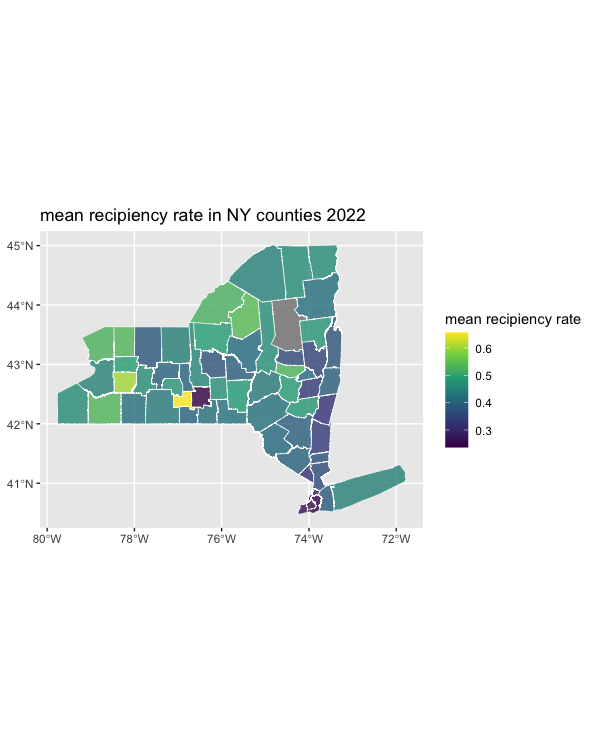
\includegraphics[width=\textwidth]{mean_recip_NY_2022.png} % Second figure
  \end{minipage}
  \caption{Spatial Summary Comparison of mean take-up rate by county; 2021(left) 2022(right)}
  \label{take-up figure}
\end{figure}

\begin{figure}[ht]
    \centering
    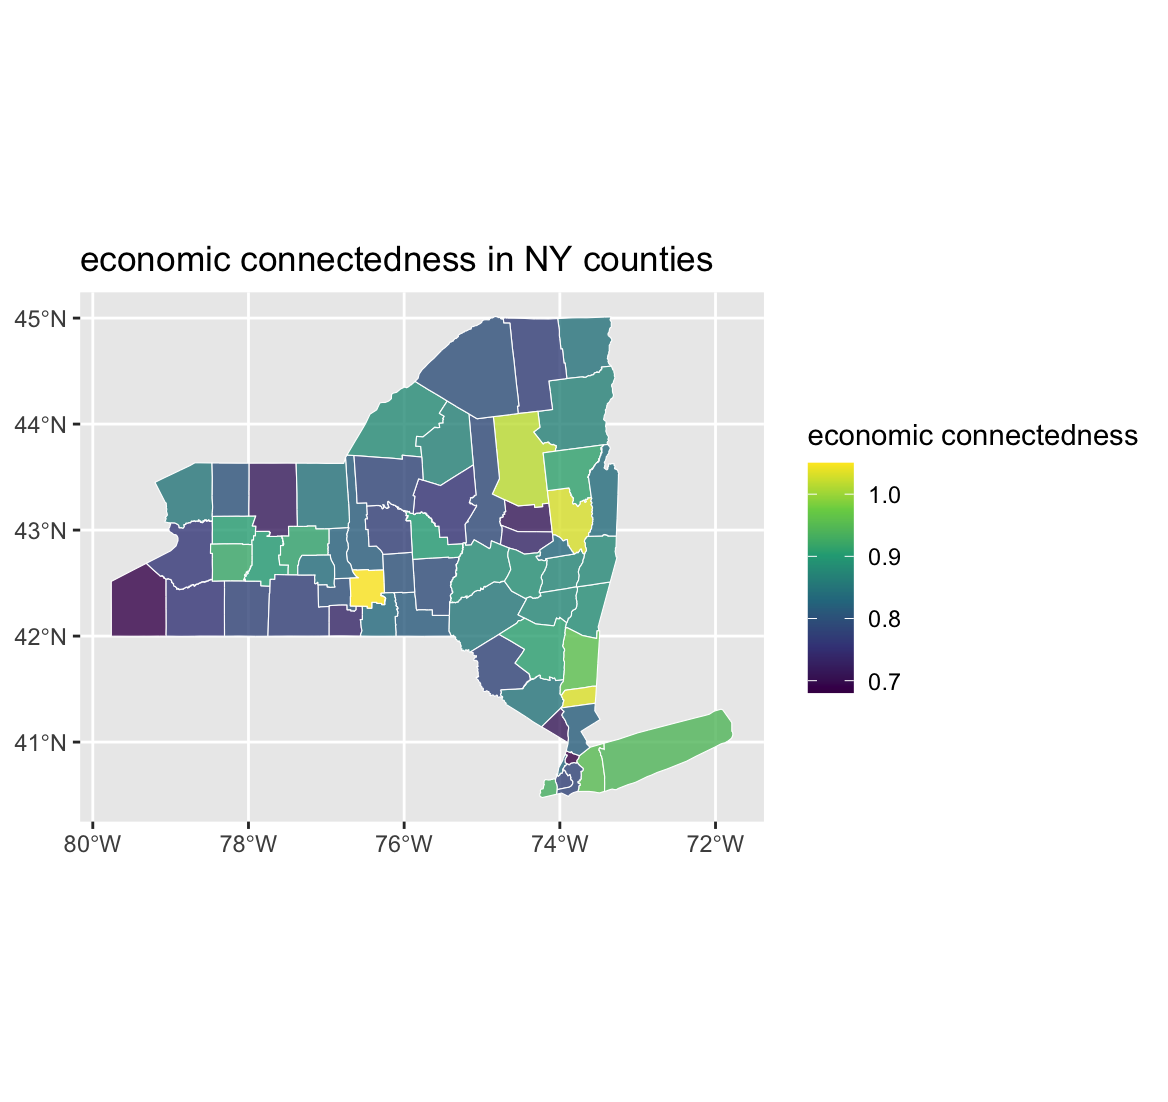
\includegraphics[width=0.8\textwidth]{ec_county_map.png}
    \caption{Spatial summary of economic connectedness}
    \label{ec figure}
\end{figure}

\begin{figure}[ht]
    \centering
    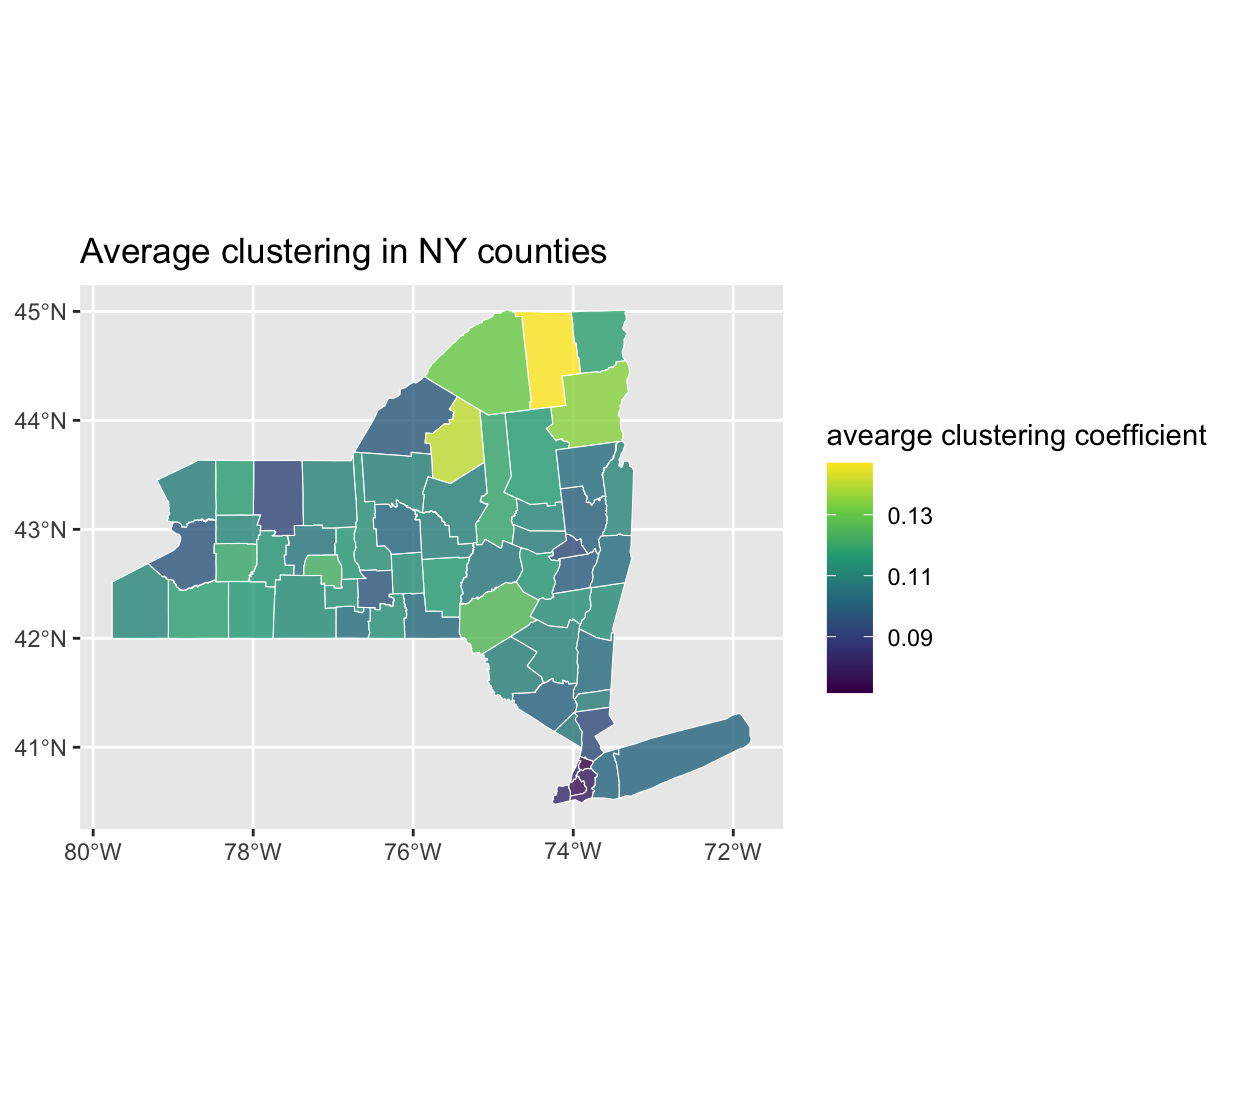
\includegraphics[width=0.8\textwidth]{clustering_map.png}
    \caption{Spatial summary of average clustering}
    \label{cluster figure}
\end{figure}

\begin{figure}[ht]
    \centering
    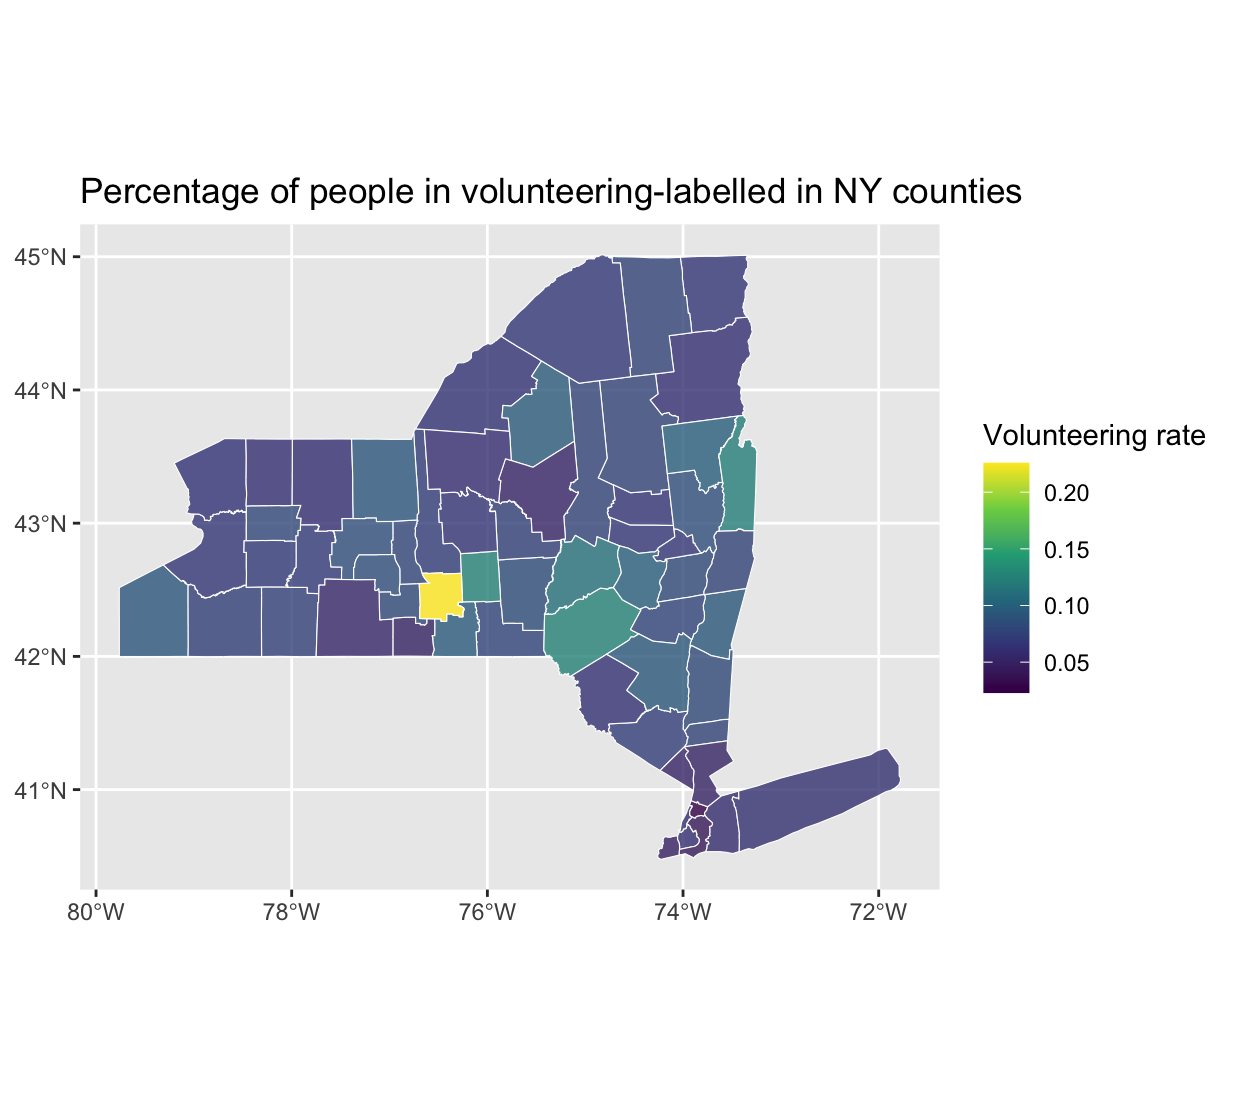
\includegraphics[width=0.8\textwidth]{volunteer_county_map.png}
    \caption{Spatial summary of average volunteering}
    \label{volun figure}
\end{figure}



\newpage



\subsection{Method}

\subsubsection{Model specification}

I am using the fixed-effect OLS model to explore the research question. In our model, two level of time fixed effects are considered. I will first only include the Year time effect and then include the month time effect.

$$Y_{\overline{\text{take-up rate}}}=\alpha_i+\beta_1 X_{sec_{it}}+\beta_2 X_{clustering_{it}}+\beta_3 X_{vonluteering_{it}}+u_{it}$$

where $\alpha_i$ is the sum of constant term and unobserved time-invariant heterogeneities across counties : $\alpha_i=\beta_0+\beta Z_i$

Assumptions:
\begin{itemize}
    \item  $u_{it}$ is not correlated with other explanatory variables
    \item $X_{1t}, X_{2t}, ... X_{nt}, ....u_{1t}, u_{2t}, ...u_{nt}$ are i.i.d. from the distribution
\end{itemize}

The base model can be expressed as a regression model containing $n-1$ dummy regressors and a constant:

$Y_{it}=\beta_0+\beta_1 X_{sec_{it}}+\beta_2 X_{clustering_{it}}+\beta_3 X_{vonlunteering_{it}}+\gamma_2 B2_t+\gamma_3 B3_t +...+\gamma_n BT_t+\mu_{it}$

\subsubsection{Dependent Variables}

The dependent variable is the monthly recipiency rate which is also known as take-up rate of UI benefits. The calculation of this recipiency rate is following: $$\text{take-up rate}=\frac{\text{Monthly continued claims}}{\text{Monthly Unemployed Population}}$$

Notice that the continued claim is also known as insured unemployment--which is the number of people who have already filed an initial claim and who have experienced a week of unemployment and then filed a continued claim to claim benefits for that week of unemployment. Continued claims data are based on the week of unmployment, not the week when the initial claim was filed. The monthly Unemployed population in specific county is just the number of people being unemployed in specific month and county (not seasonally adjusted).

\subsubsection{Explanatory Variables}

The Explanatory variables are composed of selected social capital measures from the social capital project data repository.

The first one I am using is the level of economic connectedness by the county level. The econmic connectedness is defined as the mean level of individual EC of low-SES members of that community, as follow: $$EC_c=\frac{\sum_{i\in L \cap c}{IEC_i}}{N_{Lc}}$$ where $N_{Lc}$ is the number of low-SES individuals in community c. The IEC here represents individual economic connectedness which is calculated by:

$$IEC_i=2\frac{H_i(g)}{d_i(g)}$$ where $g$ is the existing social network that social captials I am limiting on. $H_i(g)$ and $d_i(g)$ are number of high SES friend and number of total friends that individual $i$ has.

Social scientists have measured SES using many different variables, ranging from income and wealth to educational attainment, occupation, family background, neighbourhood and consumption46. To capture these varied definitions, Chetty and peer researchers compute the SES for each individual in our analysis sample by combining several measures of SES, such as average incomes in the individual’s neighbourhood and self-reported educational attainment. They combine these measures of SES into a single SES index by training a gradient-boosted regression tree model and predict the composite value for entire analysis sample. (Details can be found at the variable definition section in Methods and Supplemental Information B1 from \cite{chetty2022social1})

The second one is one of the major cohesiveness statistics at county level. It is defined as the average fraction of an individual's friend pairs who are also friends with each other.

$$Clustering_c=\frac{\sum{Clutering_i(g)}}{N_c},$$
where $Clustering_i(g)=\sum{\frac{g_{kj}}{d_i(g)(d_i(g)-1)/2}}$. $g_{kj}=1$ denotes the existence of link between individual $k$ and $j$ who are friends of $i$. and $d_i(g)$ is the degree or number of friends that individual $i$ has. Notice that I include links to people outside the county when calculating individual clustering, but only average clustering
over individuals in the relevant county to compute clustering at the
county level.

The third one is average volunteering rate by county level.  We also want to include this one because that I hypothesized that level of participating pro-social activities or being part of the volunteering group can reflect the regional take-up situations. Volunteering rate is defined as the share of Facebook users in the county who are a member of at least one volunteering or activism group. The researchers of social capital project start with the set of all Facebook Groups in the United States that are predicted to be about volunteering or activism based on their titles and do not have the privacy setting 'secret' enabled. To further improve this classification, they manually review the 50 largest such groups in the United States and the largest such group in each state, and remove the very small number of groups that are clearly misclassified. Individual-level volunteering is a binary value equal to either zero or one, they also apply noise from the Laplace($0, 1/N_\epsilon$) distribution to protect privacy. In Figure \ref{volun figure}, the spatial distribution of average volunteering rate is provided.

Here I construct Table \ref{summ stats} which provides the initial summary statistics of included variables in our regression model. For take-up rate, we have 34 missing values in the model.


\begin{table}
\centering
\begin{tabular}[h]{|m|m|m|m|m|m|m|m|m|m|}
\hline
  & n & mean & sd & median & min & max & range\\
\hline
recip\_rate & 1454 & 0.502 & 0.181 & 0.487 & 0.125 & 1.100 & 0.975\\
\hline
ec\_county & 1488 & 0.840 & 0.083 & 0.835 & 0.681 & 1.050 & 0.369\\
\hline
clustering\_county & 1488 & 0.108 & 0.014 & 0.109 & 0.072 & 0.147 & 0.075\\
\hline
volunteering\_rate\_county & 1488 & 0.076 & 0.027 & 0.073 & 0.023 & 0.226 & 0.203\\
\hline
\end{tabular}
\caption{Summary Statistics of Dependent and Independent Variables}
\label{summ stats}
\end{table}


\subsubsection{Expected Results}
It would be expected that when people in low socioeconomic status are ineligible to get insured or or unwilling to take the insurance, friendship network can be an alternative source of emergent financing and the dependency can also reduce the willingness of applying further insurance. Therefore, I hypothesize that the higher level of regional economic connectedness reduced the average take-up rate of UI benefits in a given region (county).

Higher level of regional clustering indicates the higher closeness of a community which each person knows each others' friends and which I think reduce the take-up rate because I expect more stable sub-groups of regional networks reflects less usage of institutional benefits but more interpersonal among small groups assuming that the number of unemployment is not correlated with regional clustering density.

Higher level of volunteering shows stronger inclinations toward building and sharing resources, I would expect this variable may predict more willingness in getting UI benefits from governmental programs. There are also alternative explanations to that. It is also possible the case that higher density of "volunteering" or "activism" group in a region is correlated with higher level of unemployment which could decrease the proportion of insured unemployment so that the take-up rate of UI benefits will be lower. It is also possible that area with more dense ``volunteering'' labelled group participants will have better informal support network so that less people are going to claim or get the benefits at the end therefore the take-up rate of unemployment insurance will still be lower. 

\section{Results}
\subsection{Time-fixed Effect}
Here I want to present the results of our fixed effect OLS regression model. I first only include the \textit{ec\textunderscore county} variable. Then I accumulate other interested explanatory variables to add to the regression model. From Table \ref{result1} we can see that economic connectedness at regional level is not significant when I don't add control for any possible time-related variants over time that might affect the model. And it shows that economic connectedness negatively affect the average take-up rate in the region which also matches with our hypothesis.  Table \ref{result2} shows the regression analysis results with additional variable \textit{clustering\textunderscore county}. 




\begin{table}[htbp]
   \centering
   \begin{tabular}{lccc}
      \tabularnewline \midrule \midrule
      Dependent Variable: & \multicolumn{3}{c}{Average takeup rate}\\
      Model:       & (1)           & (2)     & (3)\\  
      \midrule
      \emph{Variables}\\
      Constant     & 0.567$^{***}$ &         &   \\   
                   & (0.050)       &         &   \\   
      ec\_county   & -0.077        & -0.081  & -0.088$^{**}$\\   
                   & (0.059)       & (0.052) & (0.040)\\   
      \midrule
      \emph{Fixed-effects}\\
      Year         &               & Yes     & Yes\\  
      Month        &               &         & Yes\\  
      \midrule
      \emph{Fit statistics}\\
      Observations & 1,454         & 1,454   & 1,454\\  
      R$^2$        & 0.00119       & 0.21532 & 0.59158\\  
      Within R$^2$ &               & 0.00166 & 0.00376\\  
      \midrule \midrule
      \multicolumn{4}{l}{\emph{Heteroskedasticity-robust standard-errors in parentheses}}\\
      \multicolumn{4}{l}{\emph{Signif. Codes: ***: 0.01, **: 0.05, *: 0.1}}\\
   \end{tabular}
   \caption{Time fixed-effect model results only including ec\textunderscore county}
      \label{result1}
\end{table}

In Table \ref{result2}, the coefficient of average clustering reflects significantly positive effects on average take-up rate on UI benefits and the model fit increases as well compared to the first regression model result I provided. The results here is in the different directions of our initial hypothesis-- Suppose higher clustered region will have less needs for UI benefits thus tha take-up rates will be low. One possible explanation here is that if the level of clustering in specific regions are higher, friends and families will normally encourage people to get financial supports through public unemployment insurance program where the public insurance system are much well-developed compared to developing regions. Connecting with previous studies, given crowding out effects of formal insurance by institutions on informal insurance are minimal, it is expected that more cohesive communities can actually have positive effects on performances of public insurance program. Table \ref{result3} I used the \textit{clustering\textunderscore county} and our third included explanatory variable-\textit{volunteering\textunderscore rate\textunderscore county} here. Both \textit{clustering \textunderscore county} and \textit{volunteering\textunderscore rate\textunderscore county} produced statistically significant result in the analysis. The result from \textit{clustering\textunderscore county} follows the same effects as last analysis. The result of \textit{volunteering\textunderscore rate\textunderscore county} match with the possibly alternative explanations I offered in previous section-- the more people who belong to the volunteering group will result in less people who need to go to apply and take up the public benefits whether due to the informal support through volunteering group connections.




\begin{table}[htbp] 
   \centering
   \begin{tabular}{lccc}
      \tabularnewline \midrule \midrule
      Dependent Variable: & \multicolumn{3}{c}{Average takeup rate}\\
      Model:              & (1)          & (2)          & (3)\\  
      \midrule
      \emph{Variables}\\
      Constant            & 0.128$^{**}$ &              &   \\   
                          & (0.054)      &              &   \\   
      ec\_county          & -0.083       & -0.086$^{*}$ & -0.093$^{***}$\\   
                          & (0.054)      & (0.046)      & (0.033)\\   
      clustering\_county  & 4.11$^{***}$ & 4.06$^{***}$ & 3.97$^{***}$\\   
                          & (0.326)      & (0.297)      & (0.248)\\   
      \midrule
      \emph{Fixed-effects}\\
      Year                &              & Yes          & Yes\\  
      Month               &              &              & Yes\\  
      \midrule
      \emph{Fit statistics}\\
      Observations        & 1,454        & 1,454        & 1,454\\  
      R$^2$               & 0.09660      & 0.30832      & 0.68074\\  
      Within R$^2$        &              & 0.11999      & 0.22123\\  
      \midrule \midrule
      \multicolumn{4}{l}{\emph{Heteroskedasticity-robust standard-errors in parentheses}}\\
      \multicolumn{4}{l}{\emph{Signif. Codes: ***: 0.01, **: 0.05, *: 0.1}}\\
   \end{tabular}
     \caption{Time fixed-effect model results including ec\textunderscore county and clustering\textunderscore county}
     \label{result2}
\end{table}

\begin{table}[htbp]
   
   \centering
   \begin{tabular}{lccc}
      \tabularnewline \midrule \midrule
      Dependent Variable: & \multicolumn{3}{c}{Average takeup rate}\\
      Model:                       & (1)            & (2)            & (3)\\  
      \midrule
      \emph{Variables}\\
      Constant                     & 0.072$^{**}$   &                &   \\   
                                   & (0.034)        &                &   \\   
      clustering\_county           & 4.34$^{***}$   & 4.29$^{***}$   & 4.20$^{***}$\\   
                                   & (0.347)        & (0.315)        & (0.253)\\   
      volunteering\_rate\_county   & -0.508$^{***}$ & -0.503$^{***}$ & -0.498$^{***}$\\   
                                   & (0.163)        & (0.137)        & (0.087)\\   
      \midrule
      \emph{Fixed-effects}\\
      Year                         &                & Yes            & Yes\\  
      Month                        &                &                & Yes\\  
      \midrule
      \emph{Fit statistics}\\
      Observations                 & 1,454          & 1,454          & 1,454\\  
      R$^2$                        & 0.10076        & 0.31226        & 0.68430\\  
      Within R$^2$                 &                & 0.12500        & 0.22993\\  
      \midrule \midrule
      \multicolumn{4}{l}{\emph{Heteroskedasticity-robust standard-errors in parentheses}}\\
      \multicolumn{4}{l}{\emph{Signif. Codes: ***: 0.01, **: 0.05, *: 0.1}}\\
   \end{tabular}
   \caption{Time fixed-effect model results including cluster\textunderscore county and volunteer\textunderscore rate \textunderscore county}
   \label{result3}
\end{table}


Lastly, I include the results from Table \ref{result4} that take all explanatory variables into account. First thing I notice here is that the estimated coefficient of variable \textit{ec\textunderscore county} are now statistically insignificant at this point. Other variables' effect remains significant and same directions. This shows that average level of economic connectedness doesn't significantly relate to the regional average take-up rate of UI benefits. Reflecting back to previous models, regional average economic connectedness level does not have good explanatory power on to our dependent variable, especially after including other possible explanatory variables.

    
\begin{table}[h!]
   \centering
   \begin{tabular}{lccc}
      \tabularnewline \midrule \midrule
      Dependent Variable:  & \multicolumn{3}{c}{Average takeup rate}\\
      \hline
      Model:                       & (1)            & (2)            & (3)\\  
      \midrule
      \emph{Variables}\\
      Constant                     & 0.079          &                &   \\   
                                   & (0.060)        &                &   \\   
      ec\_county                   & -0.009         & -0.014         & -0.024\\   
                                   & (0.062)        & (0.053)        & (0.037)\\   
      clustering\_county           & 4.34$^{***}$   & 4.28$^{***}$   & 4.19$^{***}$\\   
                                   & (0.350)        & (0.318)        & (0.257)\\   
      volunteering\_rate\_county   & -0.496$^{**}$ & -0.484$^{**}$ & -0.464$^{***}$\\   
                                   & (0.188)        & (0.162)        & (0.102)\\   
      \midrule
      \emph{Fixed-effects}\\
      Year                         &                & Yes            & Yes\\  
      Month                        &                &                & Yes\\  
      \midrule
      \emph{Fit statistics}\\
      Observations                 & 1,454          & 1,454          & 1,454\\  
      R$^2$                        & 0.10077        & 0.31229        & 0.68439\\  
      Within R$^2$                 &                & 0.12503        & 0.23015\\  
      \midrule \midrule
      \multicolumn{4}{l}{\emph{Heteroskedasticity-robust standard-errors in parentheses}}\\
      \multicolumn{4}{l}{\emph{Signif. Codes: ***: 0.01, **: 0.05, *: 0.1}}\\
   \end{tabular}
   \caption{Time fixed-effect model results including all explanatory variables}
   \label{result4}
\end{table}

\newpage
\section{Discussion}
This study provides some empirical results between aggregated social capital levels and average take-up rate of unemployment insurance. 

Reflecting to the the original studies on social capitals and economic mobility, the researchers found that the social capital measures are based not solely based on the structure of the networks or individual's degree of civic engagement. Measures the combine information of network and built-up SES composite index can have stronger relationships with income mobility. In my work, when I turn the interested direction to the situations of unemployment insurance, I found that the economic connectedness doesn't really play roles in influencing the regional average take-up rate of UI insurance. 
%discuss the comparison with mobility (To summarize, measures of social capital that are based solely on the structure of the network graph (network cohesion) or purely on individuals’ civic behaviours (civic engagement) do not have robust associations with observational measures of economic mobility across areas. Measures that combine data on networks with information on SES have stronger and more stable relationships with economic mobility.); UI take-up seems less affected by the economic connectedness and...


However, there are also several limits of data usage here. I first want to talk about the limitation of the data availability here. Due to time shortage and accessibility, I don't gain access to all UI datasets across states at county level so that I choose to focus on data only from NY state. If more time and permission allowed, I would have constructed a national-level panel data so that the results can be more fruitful. Secondly, I don't have individual level data to use for our empirical analysis. The social capital panel data we end up with are already regional summary statistics based off the cleaned and calculated statistics at regional (county) level from privacy-protected individual data combined with other data sources like American Community Survey (ACS) that analyzed in social capital atlas project. And since all calculations of individual SES measures are deleted after their analysis, I have zero control of recreating the economic connectedness measures from individual level data.



%variable selection
I also faces the problems of variable selection here. Since the explanatory variables I used here are just based off the county level statistics from social atlas project's publicly available dataset, I assume that the main or basic variables are the ones I should use in the model. And there are other potential variables I haven't considered yet in the dataset they provided. For example, just economic connectedness type statistics have other sub-types of measures like: \textit{child\textunderscore ec\textunderscore county}, which defined as the childhood measure of economic connectedness that only using individual's high school friends; \textit{ec\textunderscore high\textunderscore county}, which measures the average economic connectedness among high SES individuals only; and \textit{exposure\textunderscore grp\textunderscore mem\textunderscore county}, which measures the mean exposure to high-SES individuals by county for low-SES individuals in residential block groups based on community survey data. In cohesiveness statistics, there is also an alternative \textit{supporting\textunderscore ratio\textunderscore county} statistics which directly calculate the overall frequency with which pairs of friends have at least one friend in common, focusing only on the people and friendships within that community. This study can be stronger if sensitive analysis can be conducted by replacing selected variables with other potential variables under the hood.Second, the correlation between Volunteer \textunderscore rate\textunderscore county and ec\textunderscore county is moderately positive which might cause problem of collinearity. 


%Network Endogeneity (expand
The third one is the challenges on working with network-related data. In the datasets I am interested here, the first and second explanatory variables are directly related to network measures. Especially the second one which measures the average proportion of closed triangles for each individuals. Due to the influences on networks are normally bilateral or simultaneous so that sometime it is extremely hard to set up the direction of the regression analysis. Under our circumstance, we can say that clustering statistics might have this simultaneous feedback loop with our take-up rate of UI benefits which is also known as simultaneity problem in causal analyses: the formation of social contact networks is also influenced by the unemployment and take-up situations of UI benefits.  We normally refers this as one of the endogeneity problems on networks-- predictors that are not independent from error terms in the regression performed on networks. It's also possible that I omitted the unobserved variables/attributes that both may affect the individual nodes' take-up behaviors and formation of social networks that reflecting in structural information on online social networks.

Also, the social capital data are not time-based. The calculation of social capital measures and statistics are based on the Facebook sample data collected as of May 28th, 2022. It is possible that the some statistics undergo changes in the rest of seven month however the social capital/network measures or statistics I am interested are just a single-time collection and the changes on social networks after are omitted. For dynamic point of view, since social networks are constantly changing over time, it is possible that the take-up rates is dependent on some social capital levels in previous periods but independent at current point which makes the model exogenous within current period but endogenous over time. 


If more time allowed, I may try to use different approaches to study the problems. First possible direction is to build and train a dynamic network growth model to obtain the time-series network related data not only on regional level but individual levels. And given the major problems with using traditional regression model on networks, we might need to consider other approaches like Agent-based modeling, Bayesian methods or Statistical learning. Again, by obtaining higher resolution data can increase the complexity of the problems but which actually lead to a deeper decomposition of the UI benefits take-up in social capital embedded regions.



\newpage

\printbibliography
\end{document}
